\input{../include/preamble}

\title[ID1019 A transport layer]{A transport layer}


\author{Johan Montelius}
\institute{KTH}
\date{\semester}

\begin{document}

\begin{frame}
\titlepage
\end{frame}

\begin{frame}{Communication service}

  Assume we have a communication channel that allow us to send {\em
    frames} between two connected nodes. The channel is not reliable
  so messages can be lost or delivered out of order. \pause ..... 

\vspace{20pt}
\pause We want to build a communication service that is ..... \pause better.

\pause
\vspace{20pt}

Our task is to build a communication service that provides: \pause

\begin{itemize}

\item reliable delivery: despite frames being lost \pause

\item ordered delivery: FIFO - first-in-first-out \pause

\item identity: an addressing scheme \pause

\item flow control: prevented from overflowing a receiver  

\end{itemize}


\end{frame}

\begin{frame}{layered architecture}

Build a solution using a layered architecture. 

\vspace{20pt} \pause

Each layers provides an {\em abstraction} that the layer above can make use of.

\end{frame}

\begin{frame}{layers}

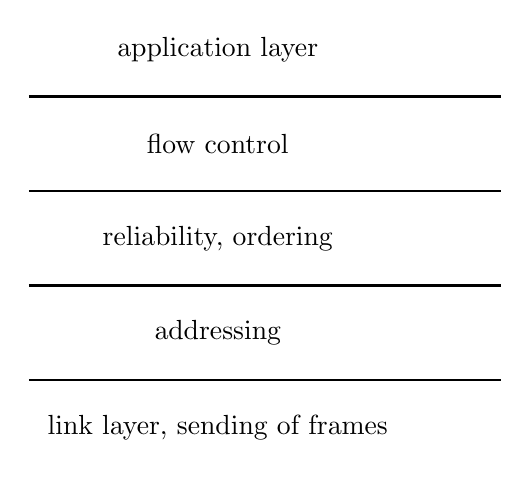
\begin{tikzpicture}[scale=0.6]

  \pause
  \node[] at (4,2) {link layer, sending of frames};

  \pause
  \draw[thick] (0,3) -- (10,3);
  \node[] at (4,4) {addressing};

  \pause
  \draw[thick] (0,5) -- (10,5);
  \node[] at (4,6) {reliability, ordering};

  \pause
  \draw[thick] (0,7) -- (10,7);

  \node[] at (4,8) {flow control};

  \pause
  \draw[thick] (0,9) -- (10,9);

  \node[] at (4,10) {application layer};

\end{tikzpicture}


\end{frame}


\begin{frame}{the link layer}


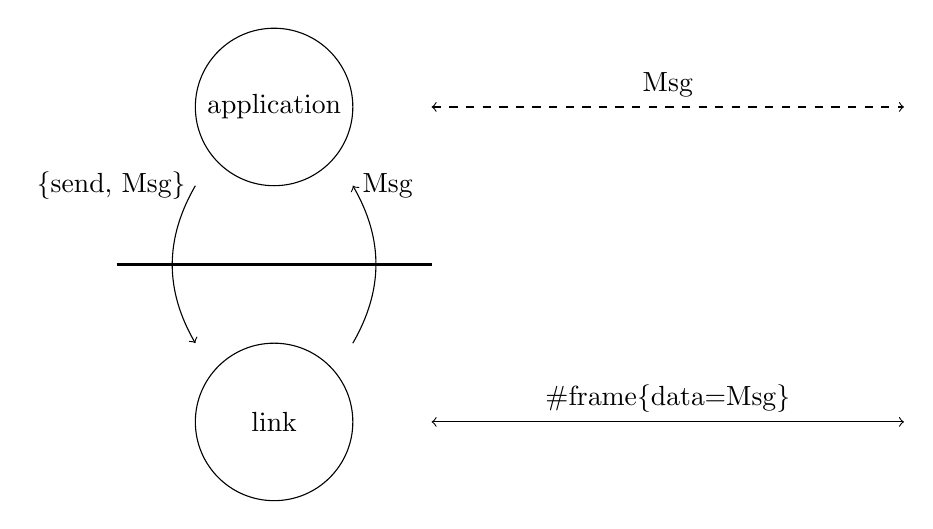
\begin{tikzpicture}

  \draw[] (2,6) circle [radius=1];
  \node[] at (2,6) {application};

  \draw[<->, dashed] (4,6) -- node[midway,above] {Msg} (10,6);

  \draw[thick] (0,4) -- (4,4);

  \draw[->] (1,5) to [in=120, out=240] (1,3);
  \draw[<-] (3,5) to [in=60, out=300] (3,3);

  \node[anchor=east] at (1,5) {\{send, Msg\}};
  \node[anchor=west] at (3,5) {Msg};

  \draw[] (2,2) circle [radius=1];
  \node[] at (2,2) {link};

  \draw[<->] (4,2) -- node[midway,above] {\#frame\{data=Msg\}} (10,2);

\end{tikzpicture}

\pause
\vspace{20pt}{\em The link layer could be extended to provide error detection and correction.}

\end{frame}



\begin{frame}{the link layer}


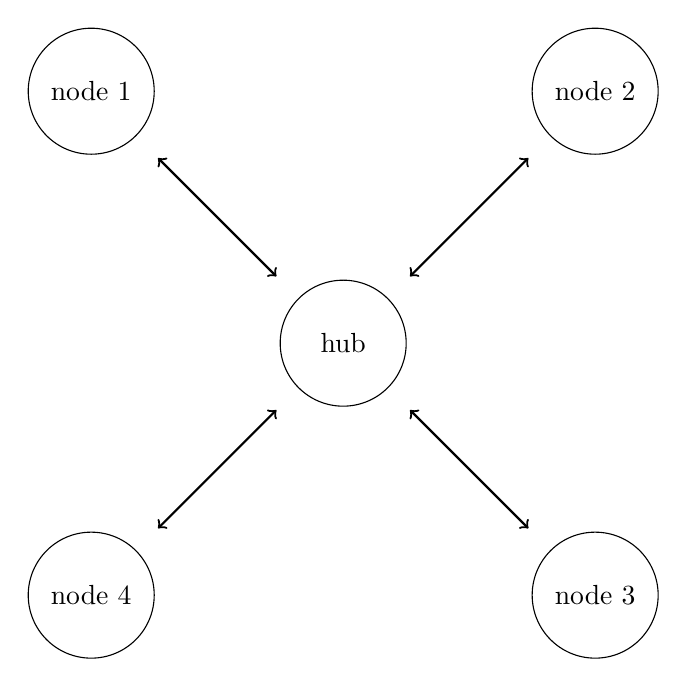
\begin{tikzpicture}[scale=0.8]

  \draw[] (5,5) circle [radius=1];
  \node[] at (5,5) {hub};

  \draw[] (1,9) circle [radius=1];
  \node[] at (1,9) {node 1};

  \draw[] (9,9) circle [radius=1];
  \node[] at (9,9) {node 2};

  \draw[] (1,1) circle [radius=1];
  \node[] at (1,1) {node 4};

  \draw[] (9,1) circle [radius=1];
  \node[] at (9,1) {node 3};

  \draw[<->, thick, shorten >=1.2cm, shorten <=1.2cm] (1,9) -- (5,5);
  \draw[<->, thick, shorten >=1.2cm, shorten <=1.2cm] (9,1) -- (5,5);
  \draw[<->, thick, shorten >=1.2cm, shorten <=1.2cm] (9,9) -- (5,5);
  \draw[<->, thick, shorten >=1.2cm, shorten <=1.2cm] (1,1) -- (5,5);

\end{tikzpicture}

\pause
\vspace{20pt}{\em The link layer will distribute any message to all all nodes.}

\end{frame}


\begin{frame}{the network layer}

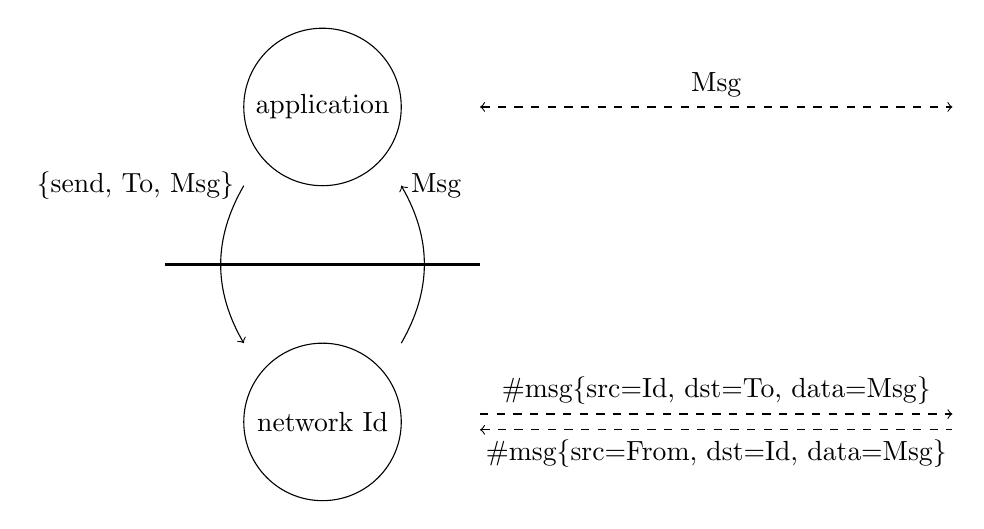
\begin{tikzpicture}

  \draw[] (2,6) circle [radius=1];
  \node[] at (2,6) {application};

  \draw[<->, dashed] (4,6) -- node[midway,above] {Msg} (10,6);

  \draw[thick] (0,4) -- (4,4);

  \draw[->] (1,5) to [in=120, out=240] (1,3);
  \draw[<-] (3,5) to [in=60, out=300] (3,3);

  \node[anchor=east] at (1,5) {\{send, To, Msg\}};
  \node[anchor=west] at (3,5) {Msg};

  \draw[] (2,2) circle [radius=1];
  \node[] at (2,2) {network Id};

  \draw[->, dashed] (4,2.1) -- node[midway,above] {\#msg\{src=Id, dst=To, data=Msg\}} (10,2.1);
  \draw[<-, dashed] (4,1.9) -- node[midway,below] {\#msg\{src=From, dst=Id, data=Msg\}} (10,1.9);

\end{tikzpicture}

\pause
\vspace{20pt}{\em The network layer will only forward messages with the right destination.}

\end{frame}

\begin{frame}{order and reliability}

\pause A {\em communication channel} is a duplex flow of an ordered sequence of messages. 

\pause 
 \vspace{20pt}
\begin{itemize}
  \item add a sequence number to each message \pause
  \item order messages as they arrive and \pause
  \item resend lost messages
\end{itemize}

\end{frame}

\begin{frame}{the network layer}

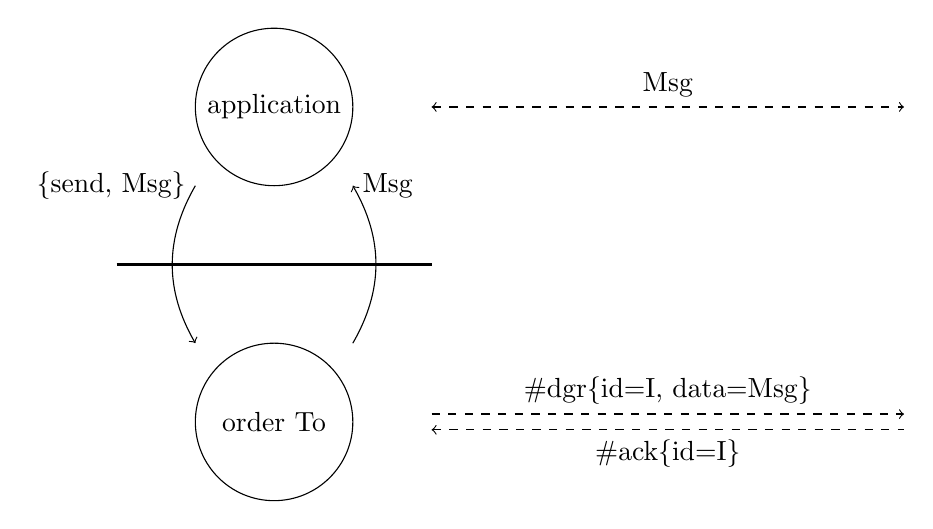
\begin{tikzpicture}

  \draw[] (2,6) circle [radius=1];
  \node[] at (2,6) {application};

  \draw[<->, dashed] (4,6) -- node[midway,above] {Msg} (10,6);

  \draw[thick] (0,4) -- (4,4);

  \draw[->] (1,5) to [in=120, out=240] (1,3);
  \draw[<-] (3,5) to [in=60, out=300] (3,3);

  \node[anchor=east] at (1,5) {\{send, Msg\}};
  \node[anchor=west] at (3,5) {Msg};

  \draw[] (2,2) circle [radius=1];
  \node[] at (2,2) {order To};

  \draw[->, dashed] (4,2.1) -- node[midway,above] {\#dgr\{id=I, data=Msg\}} (10,2.1);
  \draw[<-, dashed] (4,1.9) -- node[midway,below] {\#ack\{id=I\}} (10,1.9);

\end{tikzpicture}

\pause
\vspace{20pt}{\em The layer will need to buffer messages and use a timeout to detect missing datagrams.}

\end{frame}

\begin{frame}{flow control}

\pause

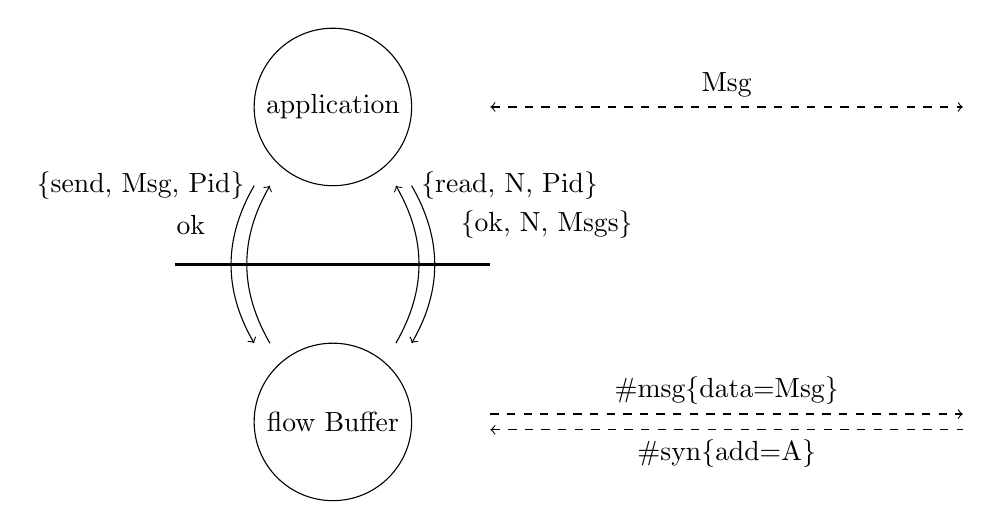
\begin{tikzpicture}

  \draw[] (2,6) circle [radius=1];
  \node[] at (2,6) {application};

  \draw[<->, dashed] (4,6) -- node[midway,above] {Msg} (10,6);

  \draw[thick] (0,4) -- (4,4);

  \draw[->] (1,5) to [in=120, out=240] (1,3);
  \node[anchor=east] at (1,5) {\{send, Msg, Pid\}};
  \draw[<-] (1.2,5) to [in=120, out=240] (1.2,3);
  \node[anchor=east] at (0.5,4.5) {ok};

  \draw[->] (3,5) to [in=60, out=300] (3,3);
  \node[anchor=west] at (3,5) {\{read, N, Pid\}};
  \draw[<-] (2.8,5) to [in=60, out=300] (2.8,3);
  \node[anchor=west] at (3.5,4.5) {\{ok, N, Msgs\}};

  \draw[] (2,2) circle [radius=1];
  \node[] at (2,2) {flow Buffer};

  \draw[->, dashed] (4,2.1) -- node[midway,above] {\#msg\{data=Msg\}} (10,2.1);
  \draw[<-, dashed] (4,1.9) -- node[midway,below] {\#syn\{add=A\}} (10,1.9);
\end{tikzpicture}


\vspace{20pt}{\em We are introducing a synchronous interface - only send if receiver prepared.}

\end{frame}


\begin{frame}{layered architecture}

\pause

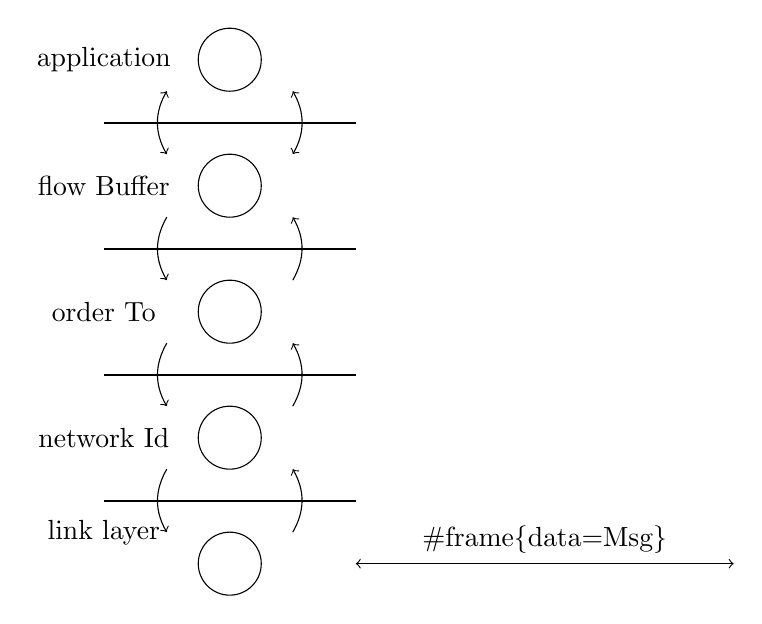
\begin{tikzpicture}[scale=0.8]

  \draw[] (2,8) circle [radius=0.5];    \node[] at (0,8) {application};

  \draw[thick] (0,7) -- (4,7);

    \draw[<->] (1,7.5) to [in=120, out=240] (1,6.5);
    \draw[<->] (3,7.5) to [in=60, out=300] (3,6.5);

  \draw[] (2,6) circle [radius=0.5];  \node[] at (0,6) {flow Buffer};

  \draw[thick] (0,5) -- (4,5);

    \draw[->] (1,5.5) to [in=120, out=240] (1,4.5);
    \draw[<-] (3,5.5) to [in=60, out=300] (3,4.5);

  \draw[] (2,4) circle [radius=0.5]; \node[] at (0,4) {order To};

  \draw[thick] (0,3) -- (4,3);
 
    \draw[->] (1,3.5) to [in=120, out=240] (1,2.5);
    \draw[<-] (3,3.5) to [in=60, out=300] (3,2.5);

  \draw[] (2,2) circle [radius=0.5];  \node[] at (0,2) {network Id};

  \draw[thick] (0,1) -- (4,1);

     \draw[->] (1,1.5) to [in=120, out=240] (1,0.5);
     \draw[<-] (3,1.5) to [in=60, out=300] (3,0.5);

  \draw[] (2,0) circle [radius=0.5];  \node[] at (0,0.5) {link layer};

  \draw[<->] (4,0) -- node[midway,above] {\#frame\{data=Msg\}} (10,0);
\end{tikzpicture}


\vspace{20pt}{\em We are introducing a synchronous interface - only send if receiver prepared.}

\end{frame}

\begin{frame}{Assignment}

\pause

\vspace{40pt}\hspace{40pt} Implement the layered communication service.

\end{frame}

\begin{frame}{Layered architecture}


\vspace{40pt}\hspace{40pt} Pros and Cons?

\end{frame}

\begin{frame}{the link layer}

\begin{tikzpicture}[>=stealth', node distance=3cm, semithick, auto]

    \node[initial, state]            (init)                              {init};
    \node[state]                     (link)    [above right of=init]     {link};
    \node[accepting, state]          (final)   [below right of=init]     {final};


    \path[->]   (init)   edge       [bend left]     node      {\{connect, Dest\}}       (link)
                         edge       [bend right]    node      {quit}          (final) 
                (link)   edge       [loop above]    node      {\{send, Msg\}}          (link)
                         edge       [loop right]    node      {\#frame\{data=Msg\}}           (link)
                         edge       [bend left]     node      {quit}          (final);
\end{tikzpicture}

\end{frame}

\begin{frame}[fragile]{the link layer}

\begin{lstlisting}
start(Master) ->
    Lnk = spawn(fun() -> init(Master) end),
    {ok, Lnk}.

init(Master) ->
    receive 
        {connect, Lnk} ->
            link(Master, Lnk);
        quit ->
            ok
    end.
\end{lstlisting}

\end{frame}


\begin{frame}[fragile]{the link layer}

\begin{lstlisting}
-record(frame, {data=[]}).

link(Master, Lnk) ->
    receive 
        {send, Msg} ->
            Lnk ! #frame{data=Msg},
            link(Master, Lnk);
        #frame{data=Msg} ->
            Master ! Msg,
            link(Master, Lnk);
        quit ->
            ok
    end.
\end{lstlisting}

\end{frame}

\begin{frame}[fragile]{a simple test}

\begin{columns}
  \begin{column}{0.6\linewidth}
    \begin{lstlisting}
test() ->
   Alice = spawn(fun()-> alice() end),
   Bob = spawn(fun()-> bob() end),
   L1 = link:start(Alice),
   L2 = link:start(Bob),
   Alice ! {connect, L1},
   Bob ! {connect, L2},
   L1 ! {connect, L2},
   L2 ! {connect, L1}.
    \end{lstlisting}
  \end{column}
  \begin{column}{0.4\linewidth}
  \end{column}    
\end{columns}
\end{frame}


\begin{frame}{extensions}

\begin{itemize}
  \item What if the link layer could only send sequences of bytes?  \pause
  \item Can we add error detection in the link layer? \pause
\end{itemize}

\end{frame}

\begin{frame}[fragile]{a hub}

\begin{tikzpicture}[>=stealth', node distance=3cm, semithick, auto]

    \node[initial, state]            (hub)                              {hub};
    \node[accepting, state]          (final)   [right of=hub]     {final};


    
    \path[->]   (hub)   edge       [loop above, every loop/.append style={looseness=10,in=100, out=160 }]     node      {\{connect, Dest\}}       (hub)
                        edge       [loop below, every loop/.append style={looseness=10,in=260, out=200 }]     node      {\{disconnect, Dest\}}    (hub)
                        edge       [loop above, every loop/.append style={looseness=6,in=20, out=80 }]     node      {\#frame\{\}}                 (hub)
                        edge       [loop below, every loop/.append style={looseness=6,in=340, out=280 }]     node      {'DOWN'}                 (hub)
                        edge       []               node       {quit}          (final);
    

\end{tikzpicture}
\end{frame}

\begin{frame}[fragile]{a hub}

\begin{lstlisting}
hub(Connected) ->
    receive 
        {connect, Pid} ->
            hub([{Ref, Pid}|Connected]);

        {disconnect, Pid} ->
            hub(lists:keydelete(Pid, 2, Connected));

        #frame{}=Frm ->
            lists:foreach(fun({_,Pid}) -> Pid ! Frm end, 
                          Connected),
            hub(Connected);
        end.
\end{lstlisting}
\end{frame}


\begin{frame}[fragile]{network layer}

\begin{tikzpicture}[>=stealth', node distance=3cm, semithick, auto]

    \node[initial, state]            (init)                              {init Id};
    \node[state]            (net)    [above right of=init]               {net Id};
    \node[accepting, state]          (final)   [below right of=init]     {final};

    
    \path[->]   (init)   edge       [bend left]     node      {\{connect, Lnk\}}       (net)
                         edge       [] node {quit} (final)
                (net)    edge       [loop above, every loop/.append style={looseness=10,in=20, out=80 }]     node[anchor=west]      {\#msg\{dst=Id, msg=Msg\}}     (net)
                         edge       [loop above, every loop/.append style={looseness=10,in=100, out=160 }]     node[anchor=east]      {\{send, To, Msg\}}     (net)
                         edge       [loop below, every loop/.append style={looseness=6,in=340, out=280 }]     node      {\#msg\{\}}     (net)
                         edge       []               node       {quit}          (final);
    
\end{tikzpicture}

\end{frame}


\begin{frame}[fragile]{network layer}

\begin{lstlisting}
network(Master, Id, Link) ->
    receive
        {send, To, Msg} ->
            Link ! {send, #msg{src=Id, dst=To,  data=Msg}},
            network(Master, Id, Link);
        #msg{dst=Id, data=Msg} ->
            Master ! Msg,
            network(Master, Id, Link);
        #msg{}=_ ->
            network(Master, Id, Link);
        quit ->
            ok
    end.
\end{lstlisting}

\end{frame}

\begin{frame}{an extension}

\begin{itemize}
  \item Could we build a switch or router? \pause
\end{itemize}

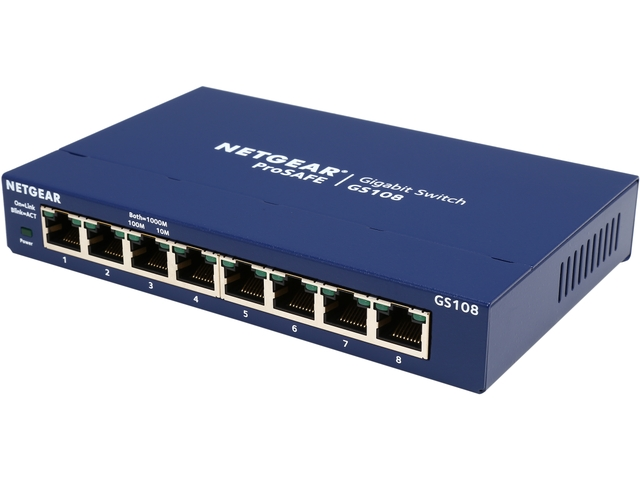
\includegraphics[scale=0.4]{switch.jpg}

\end{frame}

\begin{frame}[fragile]{a first try}

\begin{columns}
 \begin{column}{0.4\linewidth}
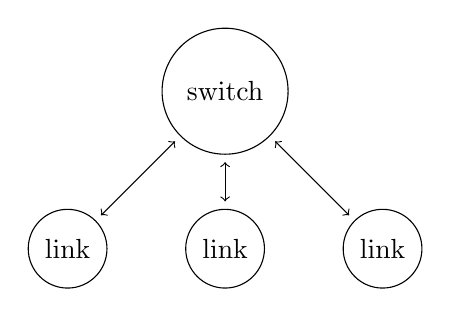
\begin{tikzpicture}
  \draw[] (4,6) circle [radius=0.8];    \node[] at (4,6) {switch};

\pause

  \draw[] (2,4) circle [radius=0.5];    \node[] at (2,4) {link};
  \draw[] (4,4) circle [radius=0.5];    \node[] at (4,4) {link};
  \draw[] (6,4) circle [radius=0.5];    \node[] at (6,4) {link};

  \draw[<->, shorten <=0.6cm, shorten >=0.9cm] (2,4) -- (4,6);
  \draw[<->, shorten <=0.6cm, shorten >=0.9cm] (4,4) -- (4,6);
  \draw[<->, shorten <=0.6cm, shorten >=0.9cm] (6,4) -- (4,6);

\end{tikzpicture}
 \end{column}
 \begin{column}{0.6\linewidth}
   \begin{lstlisting}
switch(Links) ->
    receive
        #msg{src=Src, dst=Dst}=Msg ->
             :
             forward message 
             to the right link ..
             :
             switch(Links);

    end.
   \end{lstlisting}
 \end{column}
\end{columns}

\end{frame}

\begin{frame}[fragile]{a second try}

  \begin{columns}
    \begin{column}{0.4\linewidth}
      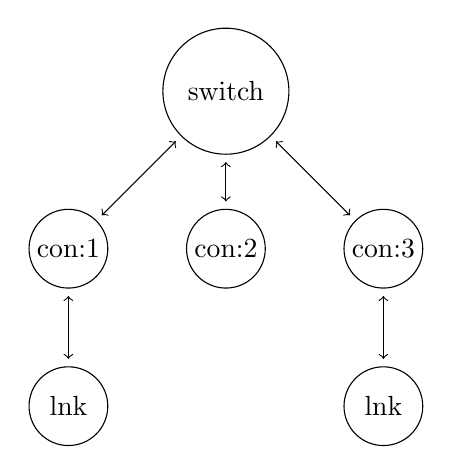
\begin{tikzpicture}
  \draw[] (4,6) circle [radius=0.8];    \node[] at (4,6) {switch};

\pause

  \draw[] (2,4) circle [radius=0.5];    \node[] at (2,4) {con:1};
  \draw[] (4,4) circle [radius=0.5];    \node[] at (4,4) {con:2};
  \draw[] (6,4) circle [radius=0.5];    \node[] at (6,4) {con:3};

  \draw[<->, shorten <=0.6cm, shorten >=0.9cm] (2,4) -- (4,6);
  \draw[<->, shorten <=0.6cm, shorten >=0.9cm] (4,4) -- (4,6);
  \draw[<->, shorten <=0.6cm, shorten >=0.9cm] (6,4) -- (4,6);

\pause

  \draw[] (2,2) circle [radius=0.5];    \node[] at (2,2) {lnk};
  \draw[<->, shorten <=0.6cm, shorten >=0.6cm] (2,2) -- (2,4);

\pause

  \draw[] (6,2) circle [radius=0.5];    \node[] at (6,2) {lnk};
  \draw[<->, shorten <=0.6cm, shorten >=0.6cm] (6,2) -- (6,4);
       \end{tikzpicture}
    \end{column}

    \begin{column}{0.6\linewidth}
       \begin{lstlisting}
switch(Cache, All) ->
    receive

       {frw, Src, Dst, From, Msg} ->
             :
             remember that messages to 
             Src should go to From
             :
             forward the message Msg
             to the right connection
             :
             switch(Updated, All);
    end.
       \end{lstlisting}
    \end{column}
  \end{columns}
\end{frame}

\begin{frame}[fragile]{a new connection}

  \begin{columns}
    \begin{column}{0.4\linewidth}
      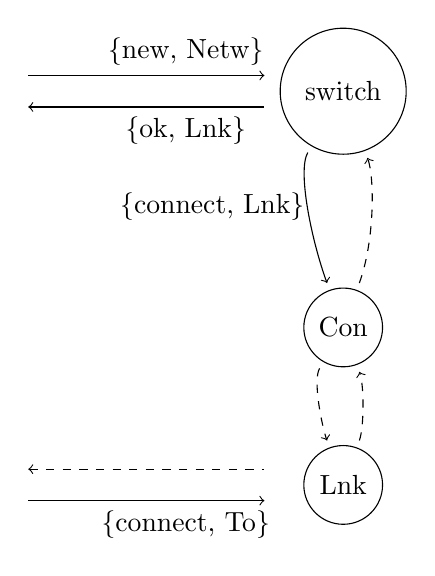
\begin{tikzpicture}
  \draw[] (4,6) circle [radius=0.8];    \node[] at (4,6) {switch};

  \draw[->, shorten >=1cm] (0,6.2) -- node[midway,above] {\{new, Netw\}} (4,6.2);
\pause

  \draw[] (4,3) circle [radius=0.5];    \node[] at (4,3) {Con};

  \draw[->, dashed, shorten <=0.6cm, shorten >=0.9cm] (4,3) to [in=290, out=70]  (4,6);

\pause

  \draw[] (4,1) circle [radius=0.5];    \node[] at (4,1) {Lnk};
  \draw[->, dashed, shorten <=0.6cm, shorten >=0.6cm] (4,1) to [in=290, out=70]  (4,3);

\pause

  \draw[->, shorten <=0.9cm, shorten >=0.6cm] (4,6) to [out=240, in=110]  node[midway,left, anchor=east] {\{connect, Lnk\}} (4,3);

\pause

  \draw[->, dashed, shorten <=0.6cm, shorten >=0.6cm] (4,3) to [in=110, out=240]  (4,1);

\pause

  \draw[<-, shorten >=1cm] (0,5.8) -- node[midway,below] {\{ok, Lnk\}} (4,5.8);

\pause

  \draw[->, shorten >=1cm] (0,0.8) -- node[midway,below] {\{connect, To\}} (4,0.8);

\pause

  \draw[<-, dashed, shorten >=1cm] (0,1.2) --  (4,1.2);

       \end{tikzpicture}
    \end{column}

    \begin{column}{0.6\linewidth}
       \begin{lstlisting}
switch(Cache, All) ->
    receive

        {new, Netw} ->
            Self = self(),
            Con = spawn(fun()-> connection(Self) end),
            {ok, Lnk} = link:start(Con),
            Con ! {connect, Link},
            Netw ! {ok, Lnk},
            switch(Cache, [Con|All]);
         :
    end.
       \end{lstlisting}
    \end{column}
  \end{columns}
\end{frame}


\begin{frame}{communication diagram}

\begin{tikzpicture}

  \coordinate (n0) at (0,6);
  \coordinate (nn) at (0,-0.5);

  \coordinate (a0) at (3,2);
  \coordinate (an) at (3,-0.5);

  \coordinate (b0) at (5,4);
  \coordinate (bn) at (5,-0.5);

  \coordinate (c0) at (6,5);
  \coordinate (cn) at (6,-0.5);

  \coordinate (s0) at (10,6);
  \coordinate (sn) at (10,-0.5);

  \coordinate (n1) at ($(n0)+(0,-0.5)$);
  \coordinate (s1) at ($(s0)+(0,-0.5)$);

  \draw[->] (n0) to []  (nn);
  \draw[->] (s0) to []  (sn);

  \node[anchor=south] at (n0) {Node};
  \node[anchor=south] at (s0) {Switch};

  \pause

  \draw[->, shorten <=0.2cm, shorten >=0.2cm] (n1) -- node[midway, above] {\{new, N\}} (s1);

  \pause

  \coordinate (s2) at ($(s1)+(0,-0.5)$);
  \coordinate (s3) at ($(s2)+(0,-1)$);

  \draw[dashed] (s2) -- (c0);

  \draw[dashed] (s3) -- (b0);

  \node[anchor=south] at (c0) {Con};  
  \node[anchor=south] at (b0) {Lnk1};  

  \draw[->] (c0) to []  (cn);
  \draw[->] (b0) to []  (bn);

\pause
  \coordinate (s4) at ($(s3)+(0,-1)$);
  \coordinate (c1) at ($(c0)+(0,-2)$);

  \draw[->, shorten <=0.2cm, shorten >=0.2cm] (s4) -- node[midway, above] {\{connect, Lnk1\}} (c1);

\pause

  \coordinate (s5) at ($(s4)+(0,-0.5)$);
  \coordinate (n2) at ($(n1)+(0,-3)$);

  \draw[->, shorten <=0.2cm, shorten >=0.2cm] (s5) -- node[near end, above] {\{ok, Lnk1\}} (n2);

\pause

  \draw[->] (a0) to []  (an);

  \node[anchor=south] at (a0) {Lnk2};

  \coordinate (n3) at ($(n2)+(0,-0.5)$);
  \draw[dashed] (n3) -- (a0);

\pause

  \coordinate (n4) at ($(n3)+(0,-1)$);
  \coordinate (n5) at ($(n4)+(0,-1)$);
 
  \coordinate (a1) at ($(a0)+(0,-1)$);
  \coordinate (b1) at ($(b0)+(0,-4)$);

  \draw[->, shorten <=0.2cm, shorten >=0.2cm] (n4) -- node[midway, above] {\{connect, Lnk1\}} (a1);

  \draw[->, shorten <=0.2cm, shorten >=0.2cm] (n5) -- node[midway, above] {\{connect, Lnk2\}} (b1);

\end{tikzpicture}

\end{frame}

\begin{frame}{order and reliability: sender side}
  \begin{tikzpicture}[scale=1, >=stealth', node distance=4cm, semithick, auto]
    \node[initial, state]            (init)                              {init To};
    \node[state]                     (ready)   [above right of=init]     {ready I};
    \node[state]                     (send)   [below right of=ready]      {ack A, I};
    \node[accepting, state]          (final)   [below right of=init]     {final};
    
    \path[->]   (init)   edge       [bend left]     node      {\{connect, Net\}}       (ready)
                         edge       [bend right] node[anchor=east] {quit} (final)
                (ready)  edge       [] node[anchor=west, near start]      {\{send, Msg\}}     (send)
                         edge       [loop right]  node  {\#ack\{\}}  (ready)
                         edge       [bend right]               node[anchor=east]       {quit}          (final)                   
                (send)   edge       [loop below, every loop/.append style={looseness=6,in=340, out=30 }] node[anchor=west] {timeout}     (send)   
                         edge       [bend left] node[near start]  {\#ack\{id=A\}}  (ready)
                         edge       [bend left]               node       {quit}          (final);
      \end{tikzpicture}

\end{frame}

\begin{frame}{order and reliability: receiver side}

      \begin{tikzpicture}[scale=1,>=stealth', node distance=3cm, semithick, auto]
    \node[initial, state]            (init)                              {init From};
    \node[state]                     (receive)   [above right of=init]      {receive I};
    \node[accepting, state]          (final)   [below right of=init]     {final};
    
    \path[->]   (init)   edge       [bend left]     node      {\{connect, Net\}}       (receive)
                         edge       [below, bend right] node[anchor=east] {quit} (final)
                (receive)   edge    [loop above, every loop/.append style={looseness=6,in=20, out=80 }] node[anchor=west]   {\#dgr\{id=I\}}     (receive)
                         edge       [loop below, every loop/.append style={looseness=6,in=340, out=280 }] node[anchor=west] {\#dgr\{id=J\} if $J<I$}     (receive)
                         edge       []               node       {quit}          (final);
      \end{tikzpicture}

\end{frame}


\begin{frame}{order and reliability: adding a buffer}

\begin{tikzpicture}[scale=1, >=stealth', node distance=4cm, semithick, auto]
    \node[initial, state]            (init)                              {init To};
    \node[state]                     (ready)   [above right of=init]     {ready I, A};
    \node[state]                     (send)   [below right of=ready]      {ack A, I};
    \node[accepting, state]          (final)   [below right of=init]     {final};

    
    \path[->]   (init)   edge       [bend left]     node      {\{connect, Net\}}       (ready)
                         edge       [bend right] node[anchor=east] {quit} (final)
                (ready)  edge       [] node[anchor=west, near start]      {\{send, Msg\}}     (send)
                         edge       [loop right]  node  {\#ack\{\}}  (ready)
                         edge       [bend right]               node[anchor=east]       {quit}          (final)                   
                (send)   edge       [loop above, every loop/.append style={looseness=6,in=20, out=70 }] node[anchor=west]    {\{send, Msg\}} (send)
                         edge       [loop below, every loop/.append style={looseness=6,in=310, out=0 }] node[anchor=west] {timeout}     (send)   
                         edge       [loop above, every loop/.append style={looseness=6,in=230, out=170 }] node[anchor=north] {}     (send)
                         edge       [bend left] node  {\#ack\{\}}  (ready)
                         edge       [bend left]               node       {quit}          (final);
\end{tikzpicture}

\end{frame}

\begin{frame}[fragile]{order and reliability}

  \begin{lstlisting}
order(Master, To, N, I, [], Net) ->
    receive
        #dgr{id=I, data=Msg} ->
            Net ! {send, To, #ack{id=I}},           
            Master ! Msg,
            order(Master, To, N, I+1, [], Net);
        #dgr{id=J} when J < I ->
            Net ! {send, To, #ack{id=J}},           
            order(Master, To, N, I, [], Net);
        #ack{} ->
            order(Master, To, N, I, [], Net);
        {send, Msg} ->
            Net ! {send, To, #dgr{id=N, data=Msg}},
            order(Master, To, N+1, I, [{N,Msg}], Net)
    end;
  \end{lstlisting}

\end{frame}


\begin{frame}[fragile]{order and reliability}

  \begin{lstlisting}
order(Master, To, N, I, [{A,Res}|Rest]=Buffer, Net) ->
    receive
          :              
        #ack{id=A} ->
            order(Master, To, N, I, Rest, Net);
        #ack{id=B} when B < A->
            order(Master, To, N, I, Buffer, Net);
         :
    after 10 ->
            Dgr = #dgr{id=A, data=Res},
            Net ! {send, To, Dgr},
            order(Master, To, N, I, Buffer, Net)
    end.
  \end{lstlisting}
\end{frame}


\begin{frame}{communication diagram}

\begin{tikzpicture}

  \coordinate (s0) at (0,6);
  \coordinate (sn) at (0,0);

  \coordinate (a0) at (4,6);
  \coordinate (an) at (4,0);

  \coordinate (b0) at (10,6);
  \coordinate (bn) at (10,0);

  \coordinate (r0) at (13,6);
  \coordinate (rn) at (13,0);

  \draw[->] (s0) to []  (sn);
  \draw[->] (r0) to []  (rn);
  \draw[->] (a0) to []  (an);
  \draw[->] (b0) to []  (bn);

  \node[anchor=south] at (s0) {Sender};
  \node[anchor=south] at (r0) {Receiver};
  \node[anchor=south] at (a0) {Order 1};
  \node[anchor=south] at (b0) {Order 2};

  \pause

  \coordinate (s1) at ($(s0)+(0,-0.5)$);

  \coordinate (a1) at ($(a0)+(0,-0.5)$);

  \draw[->, shorten <=0.2cm, shorten >=0.2cm] (s1) -- node[midway, above] {\{send, Msg\}} (a1);

  \pause

  \coordinate (a2) at ($(a1)+(0,-1)$);
  \coordinate (b1) at ($(b0)+(0,-1.5)$);

  \draw[->, dashed, shorten <=0.2cm, shorten >=0.2cm] (a2) -- node[midway, above] {\#dgr\{id=1\}} (b1);

  \pause

  \coordinate (b2) at ($(b1)+(0,-0.5)$);
  \coordinate (r1) at ($(r0)+(0,-2.0)$);

  \draw[->, shorten <=0.2cm, shorten >=0.2cm] (b2) -- node[midway, above] {Msg} (r1);

  \pause

  \coordinate (a3) at ($(a2)+(0,-1)$);
  \coordinate (b3) at ($(b2)+(0,-0.5)$);

  \draw[<-, dashed, shorten <=0.2cm, shorten >=0.2cm] (a3) -- node[midway, above] {\#ack\{id=1\}} (b3);

\end{tikzpicture}

\end{frame}

\begin{frame}{communication diagram}

\begin{tikzpicture}

  \coordinate (s0) at (0,6);
  \coordinate (sn) at (0,0);

  \coordinate (a0) at (4,6);
  \coordinate (an) at (4,0);

  \coordinate (b0) at (10,6);
  \coordinate (bn) at (10,0);

  \coordinate (r0) at (13,6);
  \coordinate (rn) at (13,0);

  \draw[->] (s0) to []  (sn);
  \draw[->] (r0) to []  (rn);
  \draw[->] (a0) to []  (an);
  \draw[->] (b0) to []  (bn);

  \node[anchor=south] at (s0) {Sender};
  \node[anchor=south] at (r0) {Receiver};
  \node[anchor=south] at (a0) {Order 1};
  \node[anchor=south] at (b0) {Order 2};

  \pause

  \coordinate (s1) at ($(s0)+(0,-0.5)$);

  \coordinate (a1) at ($(a0)+(0,-0.5)$);

  \draw[->, shorten <=0.2cm, shorten >=0.2cm] (s1) -- node[midway, above] {\{send, Msg\}} (a1);

  \coordinate (a2) at ($(a1)+(0,-1)$);
  \coordinate (b1) at ($(b0)+(0,-1.5)$);

  \draw[->, dashed, shorten <=0.2cm, shorten >=0.2cm] (a2) -- node[midway, above] {\#dgr\{id=1\}} (b1);

  \coordinate (b2) at ($(b1)+(0,-0.5)$);
  \coordinate (r1) at ($(r0)+(0,-2.0)$);

  \draw[->, shorten <=0.2cm, shorten >=0.2cm] (b2) -- node[midway, above] {Msg} (r1);

  \coordinate (b3) at ($(b2)+(0,-0.5)$);

  \draw[dashed, shorten <=0.2cm, shorten >=0.2cm] (b3) -- node[near end, above] {lost} ($(b3)+(-4,0)$);

\pause

  \coordinate (a3) at ($(a2)+(0,-2)$);

  \draw[] ($(a3)-(0.5,0)$) --  ($(a3)+(0.5,0)$);

  \node[anchor=east]  at  ($(a3)-(0.5,0)$) {timeout};
 
\pause

  \coordinate (a4) at ($(a3)+(0,-1)$);
  \coordinate (b4) at ($(b3)+(0,-2)$);

  \draw[->, dashed, shorten <=0.2cm, shorten >=0.2cm] (a4) -- node[midway, above] {\#dgr\{id=1\}} (b4);

  \coordinate (a5) at ($(a4)+(0,-1)$);
  \coordinate (b5) at ($(b4)+(0,-1)$);

  \draw[<-, dashed, shorten <=0.2cm, shorten >=0.2cm] (a5) -- node[midway, above] {\#ack\{id=1\}} (b5);


\end{tikzpicture}

\end{frame}


\begin{frame}{a connection}

\pause

\vspace{40pt}

\hspace{40pt}  In our solution there is one {\em connection} per network process. \pause

\vspace{40pt}

\hspace{40pt} Could we have several connections  sharing the same network process?

\end{frame}


\begin{frame}{flow control: sender side}

\begin{tikzpicture}[scale=1, >=stealth', node distance=4cm, semithick, auto]
    \node[initial, state]            (init)                              {init};
    \node[state]                     (ready)   [above right of=init]     {ready};
    \node[state]                     (send)   [below right of=ready]     {send S};
    \node[accepting, state]          (final)   [below right of=init]     {final};

    
    \path[->]   (init)   edge       [bend left]     node      {\{connect, Net\}}       (ready)
                         edge       [bend right] node[anchor=east] {quit} (final)
                (ready)  edge       [bend right] node[anchor=east]      {\#syn\{\}}     (send)
                         edge       [bend right] node[anchor=east]       {quit}          (final)                   
                (send)   edge       [bend right] node[anchor=west]  {\{send, Msg, Pid\}}  (ready)
                         edge       [loop below, every loop/.append style={looseness=6,out=80, in=10 }] node[anchor=east] {}     (send)   
                         edge       [loop below, every loop/.append style={looseness=6,out=340, in=280 }] node[anchor=north] {\#syn\{\}}     (send)
                         edge       [bend left]               node       {quit}          (final);
\end{tikzpicture}

\end{frame}

\begin{frame}{flow control: receiver side}
\begin{tikzpicture}[scale=1,>=stealth', node distance=3cm, semithick, auto]
    \node[initial, state]            (init)                              {init Size};
    \node[state]                     (receive)   [above right of=init]      {receive S};
    \node[accepting, state]          (final)   [below right of=init]     {final};

    
    \path[->]   (init)   edge       [bend left]     node      {\{connect, Net\}}       (receive)
                         edge       [below, bend right] node[anchor=east] {quit} (final)
                (receive) edge    [loop above, every loop/.append style={looseness=6,in=20, out=80 }] node[anchor=west]   {\#msg\{data=Msg\}}     (receive)
                         edge    [loop above, every loop/.append style={looseness=6,in=300, out=0 }] node[anchor=west]   {\{read, N, Pid\}}     (receive)
                         edge       []               node       {quit}          (final);
\end{tikzpicture}
\end{frame}

\begin{frame}[fragile]{flow control}

  \begin{lstlisting}
init(Size) ->
    receive
	{connect, Net} ->
	    Net ! {send, #syn{add=Size}},
	    flow(Size, 0, [], Net)
    end.
    
flow(S, 0, Buffer, Net) ->
    receive
	#syn{add=T} ->
	    flow(S, T, Buffer, Net)
    end;
  \end{lstlisting}
\end{frame}



\begin{frame}[fragile]{flow control}

  \begin{lstlisting}
flow(S, T, [], Net) ->
    receive 
	{send, Msg, Pid} ->
	    Net ! {send, #msg{data=Msg}},
	    Pid ! ok,
	    flow(S, T-1, [], Net);
	#msg{data=Msg} ->
	    flow(S-1, T, [Msg], Net);
	#syn{add=A} ->
	    flow(S, T+A, [], Net)
    end;
  \end{lstlisting}
\end{frame}


\begin{frame}[fragile]{flow control}

  \begin{lstlisting}
flow(S, T, Buffer, Net) ->
    receive 
          :
	{read, N, Pid} ->
	    {I, Deliver, Rest} = read(N, Buffer),
	    Pid ! {ok, I, Deliver},
	    Net ! {send, #syn{add=I}},
	    flow(S+I, T, Rest, Net);
          :
    end.
  \end{lstlisting}
\end{frame}


\begin{frame}{communication diagram}


\begin{tikzpicture}

  \coordinate (s0) at (0,6);
  \coordinate (sn) at (0,0);

  \coordinate (a0) at (4,6);
  \coordinate (an) at (4,0);

  \coordinate (b0) at (10,6);
  \coordinate (bn) at (10,0);

  \coordinate (r0) at (13,6);
  \coordinate (rn) at (13,0);

  \draw[->] (s0) to []  (sn);
  \draw[->] (r0) to []  (rn);
  \draw[->] (a0) to []  (an);
  \draw[->] (b0) to []  (bn);

  \node[anchor=south] at (s0) {Sender};
  \node[anchor=south] at (r0) {Receiver};
  \node[anchor=south] at (a0) {Order 1};
  \node[anchor=south] at (b0) {Order 2};

  \pause

  \coordinate (s1) at ($(s0)+(0,-0.5)$);

  \coordinate (a1) at ($(a0)+(0,-0.5)$);


  \coordinate (a1) at ($(a0)+(0,-1)$);
  \coordinate (b1) at ($(b0)+(0,-1)$);

  \draw[<-, dashed, shorten <=0.2cm, shorten >=0.2cm] (a1) -- node[midway, above] {\#syn\{add=1\}} (b1);

\pause

  \coordinate (s1) at ($(s0)+(0,-1.5)$);
  \coordinate (a2) at ($(a1)+(0,-0.5)$);
  \draw[->, shorten <=0.2cm, shorten >=0.2cm] (s1) -- node[midway, above] {\{send, Msg1\}} (a2);

\pause

  \coordinate (a3) at ($(a2)+(0,-0.5)$);
  \coordinate (b2) at ($(b1)+(0,-1.0)$);

  \draw[->, dashed, shorten <=0.2cm, shorten >=0.2cm] (a3) -- node[midway, above] {\#msg\{data=Msg1\}} (b2);

\pause

  \coordinate (a4) at ($(a3)+(0,-0.5)$);
  \coordinate (s2) at ($(s1)+(0,-1)$);

  \draw[<-, shorten <=0.2cm, shorten >=0.2cm] (s2) -- node[midway, above] {ok} (a4);

\pause

  \coordinate (a5) at ($(a4)+(0,-0.8)$);
  \coordinate (s3) at ($(s2)+(0,-0.8)$);
  \draw[->, shorten <=0.2cm, shorten >=0.2cm] (s3) -- node[midway, above] {\{send, Msg2\}} (a5);

\pause

  \coordinate (b3) at ($(b2)+(0,-1.5)$);  
  \coordinate (r1) at ($(r0)+(0,-3.5)$);  

  \draw[<-, shorten <=0.2cm, shorten >=0.2cm] (b3) -- node[midway, above] {\{read, 2, Pid\}} (r1);

\pause

  \coordinate (b4) at ($(b3)+(0,-0.8)$);  
  \coordinate (r2) at ($(r1)+(0,-0.8)$);  

  \draw[->, shorten <=0.2cm, shorten >=0.2cm] (b4) -- node[midway, above] {\{ok, 1, [Msg1]\}} (r2);

\pause

  \coordinate (b5) at ($(b4)+(0,-0.3)$);
  \coordinate (a6) at ($(a5)+(0,-1.3)$);

  \draw[<-, dashed, shorten <=0.2cm, shorten >=0.2cm] (a6) -- node[midway, above] {\#syn\{add=1\}} (b5);

\pause

  \coordinate (b6) at ($(b5)+(0,-0.8)$);
  \coordinate (a7) at ($(a6)+(0,-0.8)$);

  \draw[->, dashed, shorten <=0.2cm, shorten >=0.2cm] (a7) -- node[midway, above] {\#msg\{data=Msg2\}} (b6);

\pause


  \coordinate (a7) at ($(a6)+(0,-1.2)$);
  \coordinate (s4) at ($(s3)+(0,-2.5)$);

  \draw[<-, shorten <=0.2cm, shorten >=0.2cm] (s4) -- node[midway, above] {ok} (a7);

\end{tikzpicture}

\end{frame}


\begin{frame}{summary}

\pause
\begin{itemize}
 \item divide a service into processes \pause
 \item layers of abstraction \pause
 \item Finite State Machine (FSM) description of a process \pause
 \item message diagrams \pause
 \item asynchronous and synchronous interfaces \pause
\end{itemize}

\vspace{20pt}{\em .. and hopefully, you have learned about communication stacks}
\end{frame}

\end{document}



